\documentclass[12pt]{book}
% \usepackage[sc]{mathpazo}
\usepackage{commands}
\hypersetup{colorlinks = true}

%\let\oldphi\phi 
%\let\phi\varphi 
%\let\varphi\oldphi


\begin{document}
	
	

\begin{tikzpicture}[remember picture,overlay]
	% If a chapter image has been specified
	\expandafter\ifstrequal\expandafter{\thechapterimage}{}{}{
		% Output the chapter image
		\node[
		anchor=north west, % Anchor point on the image
		inner sep=0pt, % Inner padding
		] at (current page.north west) {\includegraphics[angle=90,width=\paperwidth]{Images/math4OriginalSinze.jpg}};
	}
\end{tikzpicture}
\vspace{7cm}
\heading{Theory of PDEs}

\tableofcontents

\section{Basics}
Partial differential equations relate the partial derivatives of a function to each other. For example $f$ can be a function of spacial coordinates (like $x,y,z$ in the case of Cartesian coordinates), dynamical variable (like time), or any other kind of variables (like the space of genotypes g). For example suppose that $ \Phi(x,y) $ represents the electric potential of a point charge. Such function should satisfy the Laplace equation:

\[	 \partial_{xx} \Phi + \partial_{yy} \Phi = 0.	\]
Note that the symbols $ \partial_{xx} $ and $ \partial_{yy} $ are short symbols for $ \frac{\partial^2}{\partial x^2} $ and $ \frac{\partial^2}{\partial y^2} $ respectively.

\begin{defbox}{Order of PDE}
	The order of a PDE is the highest derivative that occurs in the equation. 
\end{defbox}

Based on the definition above, the Laplace equation is a second order partial differential equation. 

\subsection{Classification of The Second Order PDEs }

There are three categories of the second order PDEs that every other type of a second order PDE can be converted to one of these kinds. The most general type of a second order PDE can be written as:

\begin{equation}
	A \partial_{xx} u + B \partial_{xy} u + C \partial_{yy} u + D \partial_{x} u + E \partial_{y} u + F u = k
	\label{equ:GeneralSecondOrderPDE}
\end{equation}

In which the coefficients are all a function of $x,y$ (but not $ u $ in which case the PDE will be nonlinearx). Equation \ref{equ:GeneralSecondOrderPDE} can be summarized in a more compact form using the derivative operator $ \operatorname{L} $: 

\[	 \operatorname{L} u = 0,	\]

in which:

\[  \operatorname{L} = A \partial_{xx} + B \partial_{xy} + C \partial_{yy} + D \partial_{x} + E \partial_{y} + F \].

Because of the similarities of the equation \ref{equ:GeneralSecondOrderPDE} with the generic quadratic equation describing the conic sections, we call each class of second order PDEs with its corresponding conic section. The generic equation describing the conic sections is:

\begin{equation}
	A x^2 + B x y + C y^2 + D x + E y + K = 0.
	\label{equ:ConicSections}
\end{equation}


All of the conic sections (ellipse, parabola, hyperbola) can be described with the equation \ref{equ:ConicSections} which is determined with the discriminant $ \Delta = B^2 - 4 A C $. for $ \Delta=0 $, $ \Delta > 0 $, and $ \Delta < 0 $ the conic section will be \textbf{parabolic}, \textbf{hyperbolic}, and \textbf{elliptic} respectively. Table \ref{tab:PDE-types} summarizes special categories of the linear second order PDEs that frequently occur in physical applications. \newline


\begin{table}[]
	\centering
	\resizebox{\textwidth}{!}{%
		\begin{tabular}{|c|c|c|c|c|}
			\hline
			PDE                     & Analogous conic sec. & $\Delta$     & Class      & Application               \\ \hline
			$ u_t = u_{xx}$         & $T = x^2$           & 0            & parabolioc & Diffusion - Heat Equation \\ \hline
			$ u_{tt} = u_{xx} $     & $T^2 = x^2$         & $\Delta > 0$ & Hyperbolic & Wave Equation             \\ \hline
			$ u_{xx} + u_{yy} = 0 $ & $x^2 + y^2 = 0$ & \multirow{2}{*}{$\Delta < 0$} & \multirow{2}{*}{Elliptic} & Laplace \\ \cline{1-2} \cline{5-5} 
			$ u_{xx} + u_{yy} = c $ & $x^2 + y^2 = k$     &              &            & Poisson                   \\ \hline
		\end{tabular}%
	}
	\caption{A summary of the three class of second order linear PDE.}
	\label{tab:PDE-types}
\end{table}


\subsection{Intuitive Derivation of the Second Order PDEs}
The three classes of the second order linear PDEs in table \ref{tab:PDE-types} can be derived intuitively using the continuity law (conservation law) and the constitutive law that is determined by the nature of the problem which is the subject of the following sections. 
 
\subsubsection{Continuity Equation or Conservation Laws}
The most important part of deriving the PDE equations is the continuity law or conservation law. This fact is imposed because of our common sense about nature. Suppose that we want to study the concentration of of a red ink in a infinitesimal cube. The continuity equation, in simple terms, state that the change of the concentration of the ink inside the infinitesimal cube is equal to the ink that has entered the cube from outside from its boundaries (we are assuming no source or sink of ink inside the cube). For instance, consider the infinitesimal box in figure \ref{fig:infbox}. The change of the concentration of the ink inside the cube is $\frac{\partial c}{\partial t}$. Because we know that there are no sources or sinks of ink inside the cube, then the change in the concentration is equal to the amount that comes in and goes out from the boundaries of the box. To put this in numbers, we introduce the important vector quantity \emph{flux} $ \Phi $. Flux is the amount of particles flow per unit area per unit time (see figure \ref{fig_fluxCrossSection}).


\begin{figure}[h!]
	\centering
	\tikzset{every picture/.style={line width=0.75pt}} %set default line width to 0.75pt        
	
	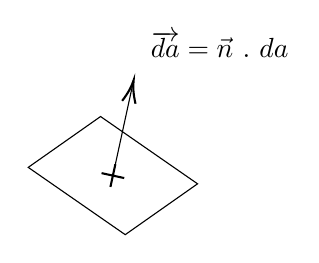
\begin{tikzpicture}[x=0.75pt,y=0.75pt,yscale=-1,xscale=1]
		%uncomment if require: \path (0,300); %set diagram left start at 0, and has height of 300
		
		%Flowchart: Data [id:dp7886171984971329] 
		\draw   (233.06,82.54) -- (279.79,114.96) -- (244.94,139.46) -- (198.21,107.04) -- cycle ;
		%Straight Lines [id:da19634912279776984] 
		\draw    (239,111) -- (248.58,66.95) ;
		\draw [shift={(249,65)}, rotate = 102.26] [color={rgb, 255:red, 0; green, 0; blue, 0 }  ][line width=0.75]    (10.93,-3.29) .. controls (6.95,-1.4) and (3.31,-0.3) .. (0,0) .. controls (3.31,0.3) and (6.95,1.4) .. (10.93,3.29)   ;
		\draw [shift={(239,111)}, rotate = 282.26] [color={rgb, 255:red, 0; green, 0; blue, 0 }  ][line width=0.75]    (-5.59,0) -- (5.59,0)(0,5.59) -- (0,-5.59)   ;
		
		% Text Node
		\draw (256,40) node [anchor=north west][inner sep=0.75pt]   [align=left] {$\displaystyle \overrightarrow{da} =\vec{n} \ .\ da$};
	\end{tikzpicture}
	\caption{The dot product $\protect\overrightarrow{\Phi}.\protect\overrightarrow{da}$ is the amount of particles passing through the infinitesimal cross section in unit time.}
	\label{fig_fluxCrossSection}
\end{figure}


\begin{figure}[h!]
	\centering
	\tikzset{every picture/.style={line width=0.75pt}} %set default line width to 0.75pt        
	
	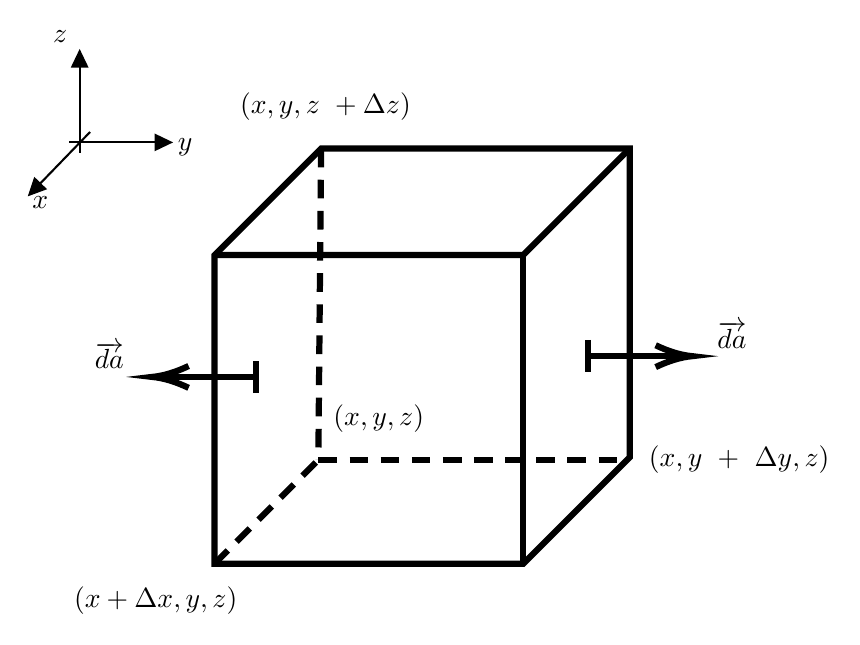
\begin{tikzpicture}[x=0.75pt,y=0.75pt,yscale=-1,xscale=1]
		%uncomment if require: \path (0,300); %set diagram left start at 0, and has height of 300
		
		%Shape: Cube [id:dp6052690098400888] 
		\draw  [line width=2.25]  (200,101.31) -- (251.31,50) -- (400,50) -- (400,198.69) -- (348.69,250) -- (200,250) -- cycle ; \draw  [line width=2.25]  (400,50) -- (348.69,101.31) -- (200,101.31) ; \draw  [line width=2.25]  (348.69,101.31) -- (348.69,250) ;
		%Straight Lines [id:da6838346844891714] 
		\draw [line width=2.25]  [dash pattern={on 6.75pt off 4.5pt}]  (250,200) -- (400,200) ;
		%Straight Lines [id:da4358863669422177] 
		\draw [line width=2.25]  [dash pattern={on 6.75pt off 4.5pt}]  (251.31,50) -- (250,200) ;
		%Straight Lines [id:da8699451449684632] 
		\draw [line width=2.25]  [dash pattern={on 6.75pt off 4.5pt}]  (200,250) -- (250,200) ;
		%Straight Lines [id:da6153923820857115] 
		\draw [line width=2.25]    (220,160) -- (174,160) ;
		\draw [shift={(170,160)}, rotate = 360] [color={rgb, 255:red, 0; green, 0; blue, 0 }  ][line width=2.25]    (17.49,-5.26) .. controls (11.12,-2.23) and (5.29,-0.48) .. (0,0) .. controls (5.29,0.48) and (11.12,2.23) .. (17.49,5.26)   ;
		\draw [shift={(220,160)}, rotate = 360] [color={rgb, 255:red, 0; green, 0; blue, 0 }  ][line width=2.25]    (0,7.83) -- (0,-7.83)   ;
		%Straight Lines [id:da3502060568264709] 
		\draw [line width=2.25]    (380,150) -- (426,150) ;
		\draw [shift={(430,150)}, rotate = 180] [color={rgb, 255:red, 0; green, 0; blue, 0 }  ][line width=2.25]    (17.49,-5.26) .. controls (11.12,-2.23) and (5.29,-0.48) .. (0,0) .. controls (5.29,0.48) and (11.12,2.23) .. (17.49,5.26)   ;
		\draw [shift={(380,150)}, rotate = 180] [color={rgb, 255:red, 0; green, 0; blue, 0 }  ][line width=2.25]    (0,7.83) -- (0,-7.83)   ;
		%Straight Lines [id:da8422422028495438] 
		\draw [line width=0.75]    (140,42) -- (112.09,70.84) ;
		\draw [shift={(110,73)}, rotate = 314.06] [fill={rgb, 255:red, 0; green, 0; blue, 0 }  ][line width=0.08]  [draw opacity=0] (8.93,-4.29) -- (0,0) -- (8.93,4.29) -- cycle    ;
		%Straight Lines [id:da7449366310627421] 
		\draw [line width=0.75]    (135,52) -- (135,5) ;
		\draw [shift={(135,2)}, rotate = 90] [fill={rgb, 255:red, 0; green, 0; blue, 0 }  ][line width=0.08]  [draw opacity=0] (8.93,-4.29) -- (0,0) -- (8.93,4.29) -- cycle    ;
		%Straight Lines [id:da9487980467676893] 
		\draw [line width=0.75]    (130,47) -- (177,47) ;
		\draw [shift={(180,47)}, rotate = 180] [fill={rgb, 255:red, 0; green, 0; blue, 0 }  ][line width=0.08]  [draw opacity=0] (8.93,-4.29) -- (0,0) -- (8.93,4.29) -- cycle    ;
		
		% Text Node
		\draw (256,172) node [anchor=north west][inner sep=0.75pt]   [align=left] {$\displaystyle ( x,y,z)$};
		% Text Node
		\draw (131,260) node [anchor=north west][inner sep=0.75pt]   [align=left] {$\displaystyle ( x+\Delta x,y,z)$};
		% Text Node
		\draw (408,192) node [anchor=north west][inner sep=0.75pt]   [align=left] {$\displaystyle ( x,y\ +\ \Delta y,z)$};
		% Text Node
		\draw (211,22) node [anchor=north west][inner sep=0.75pt]   [align=left] {$\displaystyle ( x,y,z\ +\Delta z)$};
		% Text Node
		\draw (111,72) node [anchor=north west][inner sep=0.75pt]   [align=left] {$\displaystyle x$};
		% Text Node
		\draw (181,44) node [anchor=north west][inner sep=0.75pt]   [align=left] {$\displaystyle y$};
		% Text Node
		\draw (121,-8) node [anchor=north west][inner sep=0.75pt]   [align=left] {$\displaystyle z$};
		% Text Node
		\draw (141,142) node [anchor=north west][inner sep=0.75pt]   [align=left] {$\displaystyle \overrightarrow{da}$};
		% Text Node
		\draw (441,132) node [anchor=north west][inner sep=0.75pt]   [align=left] {$\displaystyle \overrightarrow{da}$};
		
		
	\end{tikzpicture}
	\caption{The infinitesimal cube for deriving the continuity equation}
	\label{fig:infbox}
\end{figure}



\newpage

Let's get back to the infinitesimal cube in figure \ref{fig:infbox} and derive the continuity equation. We can start we tracking the net change in the number of particles inside the cube due to the flux in x direction:

\begin{align*}
	-\frac{dN_x}{dt} &= \Phi_x(x,y,z) . (-dz dy) + \Phi_x(x +dx, y,z) . (dzdy) \\
	 				&= (\Phi_x(x+dx,y,z)-\Phi_x(x,y,z))dydz 
\end{align*}

Note that the negative sign in the LHS of the equation above is simply to match the meaning of the two sides of the equations. For instance, if the RHS of the equation above is positive, it means that the net change of the number of particles in the box in negative (meaning that particles are leaving the box) which is equivalent to $ -\frac{dN}{dt} $. Similarly in the y and z direction:

\begin{align*}
	-\frac{dN_y}{dt} &= (\Phi_y(x,y+dy,z)-\Phi_y(x,y,z)) dx dz \\
	-\frac{dN_z}{dt} &= (\Phi_z(x,y,z+dz) - \Phi_z(x,y,z)) dx dy
\end{align*}

So the net change in the number of particle in the box per $dt$ will be:

\begin{align*}
	-\frac{dN}{dt} &= - (\frac{dN_x}{dt} + \frac{dN_y}{dt} + \frac{dN_z}{dt}) \\
	&= (\Phi_x(x+dx,y,z)-\Phi_x(x,y,z))dydz + \\
	&\, (\Phi_y(x,y+dy,z)-\Phi_y(x,y,z)) dx dz + \\
	&\, (\Phi_z(x,y,z+dz) - \Phi_z(x,y,z)) dx dy
\end{align*}


By dividing the both sides of the above equation by the volume of the cube $ dV = dx dy dz $ we can write:

\begin{equation*}
	\frac{dc}{dt} = - (\partial_{x}\Phi_x + \partial_{y}\Phi_y + \partial_{z}\Phi_z) = -\mathbf{\nabla} . \Phi
\end{equation*}

In which $c = N/V$ is the concentration, $ \nabla $ is the divergence operator, and $ \Phi $ is the flux. 

\begin{defbox}{Continuity Equation}
	The following important relation is known as the continuity equation(or conservation law):
	
	\begin{equation}
			\frac{dc}{dt} + \mathbf{\nabla} . \Phi = 0
	\end{equation}

	in which $\Phi$ is the flux, $c$ is the concentration, and $ \nabla $ is the divergence operator.
\end{defbox}


\subsubsection{Conservation Law for Momentum}
will be used to derive the wave equation


\subsection{Constitutive Laws: Advection, Diffusion and Wave Equation}

Having the continuity equation in hand makes the derivation PDEs very straight forward. We only need to insert the constitutive laws (which are enforced by the nature of the problem) in the continuity equations derived in the section above.


\begin{itemize}
	\item Fick's Law $\rightarrow$ Constitutive law for diffusion 
	\item Hook's law $\rightarrow$ Constitutive law for the wave equation
\end{itemize}




\chapter{Ordinary Differential Equations}

\section{Introduction}

Let's start by studying the following first order differential equation for $u$
\[ u' + mu = f, \tag{1}\]
where $m\in \R$ and $f:\R\to\R$ is a continuous function. In fact, we are trying to find a function that its derivative plus some constant times the function itself produces the function $f$. One way to tackle this problem is to multiply both sides by $e^{mx}$. Then, we will get
\[ e^{mx}u' + mue^{mx} = f e^{mx},\quad x\in \R. \]
Now the trick is to do a similar thing as completing the square in algebra, with only difference that we are aiming at completing the derivative. In other words
\[ (e^{mx} u(x))' = f(x)e^{mx}, \quad x\in\R. \]
Now by integrating both sides (or, equivalently, using the fundamental theorem of calculus) we will get
\[ e^{mx}u(x) - u(0) = \int_{0}^{x}f(s)e^{ms} ds. \]
By a little rearrangement of the terms we will get
\[ u(x) = ce^{-mx} + \int_{0}^{1}f(s)e^{m(s-x)}ds, \quad c \in \R \]
Now we can see that on only there is one function that satisfies that particular relation imposed by the differential equation, there is in fact a continuum of functions satisfying the differential equations that are parameterized by $c\in \R$. It turns out that the set of all such functions, as a set, has some very interesting properties. Let's call this set $\mathcal{A}$. As we discussed above, the elements of this set is parameterized by $c\in\R$. We can also specify this set as
\begin{equation*}
	\mathcal{A} = \set{u\ |\ u(x)=ce^{-mx} + \int_{0}^{x}f(s)e^{m(s-x)}ds\ \forall c\in \R}
\end{equation*}

\textbf{Note that we will assume that the function $f$ is Lipschitz continuous. Then we will be sure that all of the possible solutions of the ODE above are in set $\mathcal{A}$}. Studying this set more closely, reveals the fact that this set is actually a linear space, or, a vector space. This is true since
\begin{enumerate}
	\setlength\itemsep{0em}
	\item [(A1)] $u,v\in \mathcal{A} \implies u+v = v+u \in \mathcal{A}$.
	\item [(A2)] $\forall u,v,r \in \mathcal{A} \wh u+(v+r) = v+(u+r).$
	\item [(A3)] $\mathcal{O} \in \mathcal{A}$ such that $v+\mathcal{O} = \mathcal{O} + v = v$ for all $v\in \mathcal{A}$.
	\item [(A4)] $\forall v\in \mathcal{A},\ \exists u \in \mathcal{A} \st v + u = u + v = \mathcal{O}.$	
	\item []
	\item [(M1)] $\forall v \in \mathcal{A} \wh \mathcal{I}\cdot v = v\cdot \mathcal{I} = v$.
	\item [(M2)] $\forall v \in \mathcal{A} \wh \mathcal{O}\cdot v = v\cdot \mathcal{O} = \mathcal{O}$
	\item [(M3)] $\forall v\in \mathcal{A},\ a,b \in \R \wh a(bv) = (ab)v$ 
	\item []
	\item [(D1)] $\forall u,v\in \mathcal{A},\ a\in \R \wh a(u+v) = au + av.$
	\item [(D2)] $\forall u \in \mathcal{A},\ a,b\in \R \wh (a+b)u = au + bu. $
\end{enumerate}
\begin{proof}
	All of the properties of this set follows immediately from the fact that $\R$ is a vector space. To see this, see the following proof for (A1).
	Let $u,v \in \mathcal{A}$. Then $\exists c_1, c_2 \in \R$ such that 
	\[ u(x) = c_1e^{-mx} + \int_{0}^{x}f(s)e^{m(s-x)}ds, \quad v(x) = c_2e^{-mx} + \int_{0}^{x}f(s)e^{m(s-x)}ds. \]
	Thus 
	\[ (u+v)(x) = (c_1+c_2)e^{-mx} + \int_{0}^{x}f(s)e^{m(s-x)}ds. \]
	Since $c_1 + c_2 \in \R$, then $u+v \in \mathcal{A}$.
\end{proof}

So far, we have fined a set of functions $\mathcal{A}$ that solves the differential equation. However, now, we can ask for more requirement. For instance, we can ask for functions that satisfy certain initial conditions, i.e. $u(0) = u_0$. Or we can ask for functions that are defined on some interval, say $[0,1]$ that satisfy certain boundary conditions like $u(0) + u'(1) = 3$, or $u(0) = u(1)$, etc. For the case of specifying an initial condition, say $x(0) = x_0$, we can find a unique $x\in \mathcal{A}$ that solves the ODE and satisfies this initial value problem (choose $x\in \mathcal{A}$ that has $c= x_0$).


\begin{beCareful}
	Consider the following initial value problem
	\[ \dot{x} = x^{2/3}, \qquad x(0) = 0. \]
	Then at any open interval that the function $x(t)$ does not take the value 0, we can write the ODE as
	\[ \frac{\dot{x}}{x^{2/3}} = 1.  \]
	Now by integration we get the set of all solutions of the ODE 
	\[ \mathcal{A} = \set{x:[a,b]\to \R\ :\ x(t)=(\frac{x+c}{3})^3,\ x(t)\neq 0\ \forall t\in [a,b]}. \]
	Clearly, the constant solution $x(t)\equiv 0$ doe not belong to the set $\mathcal{A}$. However, we can easily verify that $x(t)\equiv 0$ is a solution to the initial value problem. So when the function $f$ is not descent enough (not Lipschitz continues in this case), then the set $\mathcal{A}$ does not contain all of the solutions for the initial value problem. So in conclusion, the initial value problem has two solutions $x(t) = t^3/3$ that belongs to $\mathcal{A}$ and $x(t) \equiv 0$ which is not in $\mathcal{A}$.\\
	However, if the function  $f$ (RHS of the initial value problem) is Lipschitz continuous, then by the Picard iteration argument we can show that there is always a unique solution that can be achieved by the integration\footnote{see the chapter 1 of the book "Ordinary Differential Equations: Qualitative Theory" by Barreira.}. 
\end{beCareful}

However, in the case of specifying boundary conditions (boundary condition problems), like demanding $u(0)=u(1)$ the situation is not as clear as the initial value problem. Given that the RHS function is Lipschitz continuous and all of the solutions of the ODE lives in the set $\mathcal{A}$, then our task is basically look for functions in $\mathcal{A}$ (which is basically isomorphic to $\R$) to see which of them satisfy the boundary condition. Then we might find no solutions, or a unique solution, or more than one solution (note the similarity with finding the solutions of a linear system $AX=B$ that based on the characterizations of the matrix $A$ we might have different scenarios for the solutions.)

Back to our example above, we find that the solutions of 
\[ u' + mu = f\] 
are all in the set
\begin{equation*}
	\mathcal{A} = \set{u\ |\ u(x)=ce^{-mx} + \int_{0}^{x}f(s)e^{m(s-x)}ds\ \forall c\in \R}
\end{equation*}
So we can determine which functions in $\mathcal{A}$ satisfies our boundary condition. This leads to the following equation
\[ c  = ce^{-m} + \int_{0}^{1}f(s)e^{m(s-1)}\ ds, \]
which implies
\[ \boxed{c = \frac{1}{1-e^{-m}}\int_{0}^{1}e^{m(s-1)}f(s)\ ds, \qquad m\neq 0}. \]
Thus when $m\neq 0$, we have a unique function in $\mathcal{A}$ that satisfies the boundary condition. However, when $m=0$, then the above equation does not make sense. Then the function $u\in \mathcal{A}$ where
\[ u(x) = c+  \int_{0}^{x}f(s)\ ds. \]
To satisfy the boundary condition, we need to have
\[ u(0) = u(1) \implies c = c+\int_{0}^{1}f(s) ds \implies \boxed{\int_{0}^{1}f(s)\ ds = 0}. \]
So in the case where $m=0$, if $\int_{0}^{1}f(s)ds=0$, then we have infinitely many solutions for the boundary value problem. But if $\int_{0}^{1}f(s)ds \neq 0$, then there is no solutions for the boundary value problem.

\begin{summary}
	Consider the following ODE
	\[ u' + mu = f. \]
	where $f$ is Lipschitz continuous. Then the set of all solutions to this ODE is 
	\[ 	\mathcal{A} = \left\{u\ |\ u(x)=ce^{-mx} + \int_{0}^{x}f(s)e^{m(s-x)}ds\ \forall c\in \R \right\}.\]
	Then for any initial value $u(0) = u_0$, we can find a unique $u\in\mathcal{A}$ that satisfies the initial value problem ($c=u_0$). However, for the boundary value problem $u(0)=u(1)$ we will have the following cases
	\begin{itemize}
		\item $m\neq 0$. Then there is a unique $u\in\mathcal{A}$ where
		\[ c = \frac{1}{1-e^{-m}}\int_{0}^{1}e^{m(s-1)}f(s)\ ds \]
		\item $m =0$. Then there are two cases
		\begin{itemize}
			\item $\int_{0}^{1}f(s)ds = 0$. We will have infinite number of solutions $\forall c\in R$ for the BVP.
			\item $\int_{0}^{1}f(s)ds \neq 0$. We will have no solutions for BVP.
		\end{itemize}
	\end{itemize}
\end{summary}

We can think about the boundary value problem in a more systematic way. First note that all the functions $u:[0,1]\to\R$ that satisfies the boundary condition $u(0) = u(1)$ for a vector space (easy to check). Thus we can think about our boundary value condition in the following way
\begin{quote}
	Let $\mathcal{B} = {u:\mathcal{C}^1([0,1],\R): u(0) = u(1) }$ be a Banach space. This is a linear space equipped with the norm $\norm{u} = \max\set{\norm{u}_\infty, \norm{u'}_\infty}$ (thus $\mathcal{B}$ is a Hilbert space). Let $Y = \mathcal{C}([0,1],\R)$ equipped with the suprimum norm. Consider for any $m\in \R$, the linear operator $L_m:X\to Y$ define as $L_mu =u'+mu$. Given any $f \in Y$ find those $u \in \mathcal{B}$ such that $L_m u = f.$
\end{quote}
If we have a unique solution, then we can write $u = \inv{L_m}f$ where $\inv{L_m}$ is the inverse operator of $L_m$. So the uniqueness of the solution is the question invertibility of the operator $L_m$. This operator is the inverse of a differential operator, thus it is an integral operator. For the specific example that we solved above, we can easily calculate this integral operator. This inverse operator exists if we have a unique solution. So we will consider the boundary value problem we solved above when $m \neq 0$. Then we know that 
\[ u(x) = ce^{-mx} + \int_{0}^{x} e^{m(s-x)}f(s)\ ds, \qquad c = \frac{1}{1-e^{-m}}\int_{0}^{1}e^{m(s-1)}f(s)ds.  \]
By substituting the value of $c$ we can write
\[  u(x) = \frac{e^{-mx}}{1-e^{-m}}\int_{0}^{1}e^{m(s-1)}f(s)\ ds  + \int_{0}^{x} e^{m(s-x)}f(s)\ ds \]
To merge the integrals into a single integral, we write 
\[  u(x) = \frac{e^{-mx}}{1-e^{-m}}\int_{0}^{1}e^{m(s-1)}f(s)\ ds  + \int_{0}^{1} H(s,x)e^{m(s-x)}f(s)\ ds \]
where $H(s,x)$ is step function with $H(s,x) = 1$ when $s< x$ and $H(s,x) = 0$ when $x<s$. Then we can write the integral above as
\[ u(x) = \int_{0}^{1}G(s,x)f(s)\ ds = \inv{L_m}f(t),\qquad
G(s,x) = \frac{1}{1-e^{-m}}\begin{cases}
	e^{m(s-x)} \quad 0<s< x<1, \\
	e^{m(s-x-1)} \quad 0<x<s<1.
\end{cases}
 \]
thus for this specific boundary value problem we have
\[ \boxed{\inv{L_m}f(t) = \int_{0}^{1} G(s,x) f(s)\ ds}. \] 
The function $G$ is called the Green's function. The Green's function can give us the exact solution of certain boundary value problems, but the most important thing about the Green's function is that it contains lots of analytic and quantitative information about the solution that we can utilize even before solving the integral\footnote{To see some of these quantitative information from the Green's function see page 4 of "Greens function in the theory of ordinary differential equations" by  Alberto Cabada.}.


\section{Construction of Green's function}
Consider the following $n$ dimensional linear boundary value problem
\[ x'(t) = A(t) x(t) + f(t), \qquad t \in J = [a,b] \tag{2.1} \]
with the boundary condition
\[ Bx(a) + Cx(b) = h, \]
where $n \in \N$, $a,b \in \R$ that $a<b$, $A \in \mathscr{L}^1(J,\mathscr{M}_{n\times n})$, $f \in \mathscr{L}^1(J,\R^n)$, $B,C \in \mathscr{M_{n\times n}}$, $h \in \R^n$, and $x \in \mathscr{AC}(J,\R^n)$. As usual, we denote by  $\mathscr{L}^1$ the set of all Lebesgue integrable function on $J$ and by $\mathscr{AC}(J,\R^n)$ the set of absolutely continuous functions on $J$. Note that $n,a,b,f,A,B,C$ and $h$ are known data of the problem.


\begin{beCareful}
	Note that we are not dealing with initial value problem, but the problem that we are looking at is boundary value problem. That is why our approach and the set of tools that we use might be different (although with some similarity). It is the nature of the problem that determines which tools we need to use. For example, for the boundary value problems, exploiting the vector space property of the set of solutions is very beneficial, whereas for the initial value problems, we exploit some other algebraic structures (the notion of flow that has a group structure) to tackle the problems. So, these two theories for boundary value and initial value problems is a very good example how to be aware of the useful structures in a problem and exploit them.
\end{beCareful}

First, we study the structure of the set of solutions of the homogeneous problem, i.e. $f\equiv 0, h\equiv 0$. Let $\mathscr{H}$ be the set of all $\mathscr{C}^1([a,b],\R^n)$ functions that satisfy the boundary condition. 
\[  \mathscr{H} = \set{f \in \mathscr{C}^1([a,b],\R^n)\ :\ Bf(a) + Cf(b) = 0}.  \]
Let $L:\mathscr{H} \to \mathscr{C}^1([a,b],\R^n)$ be an operator (differential operator) that for $u \in \mathscr{H}$ we have
\[ Lu = u' - Au. \]
Thus the set of all solutions to the homogeneous problem will be the kernel of the linear operator $L$, i.e. $u\in \mathscr{H}$ s.t. $Lu = 0$.

The following example demonstrates our discussion above on a more concrete example.

\begin{example}
	Consider the following boundary value problem
	\[ \vectt{x'(t)}{y'(t)}=\underbrace{ \matt{0}{1}{-\lambda}{0}}_{A} \vectt{x(t)}{y(t)},\qquad t\in [0,2\pi]\]
	with boundary conditions given as
	\[ \underbrace{\matt{0}{1}{0}{0}}_{B}\vectt{x(0)}{y(0)} + \underbrace{\matt{0}{0}{0}{1}}_{C} \vectt{x(2\pi)}{y(2\pi)} = \vectt{0}{0}. \]
	We can write this in a much more compact vector form
	\[ \Phi'(t) = A\Phi(t), \qquad B\Phi(0) + C\Phi(2\pi) = 0. \tag{E.2.1}\]
	where $\Phi:[0,2\pi]\to \R^2$. Observe that the solutions of this system of ODEs is the same as the solutions for the second order ODE $x'' = -\lambda x$. Denote the set of all differentiable functions that satisfy the boundary condition as $\mathscr{H}$.
	\[ \mathscr{H} = \set{\Phi \in \mathscr{C}^1([0,1],\R^2)\ :\ B\Phi(0) + C\Phi(2\pi) = \mathscr{O} }. \]
	where $\mathscr{O}$ is a $\mathscr{C}^1$ function that is identically zero $\mathscr{O}(t)\equiv0$. Define the differential operator $L: \mathscr{H} \to \mathscr{C}^1([0,2\pi],\R^2)$ to be
	\[ L \Phi = \Phi' - A \Phi, \qquad \Phi \in \mathscr{H}. \]
	
	 Now Depending on the value of $\lambda$, the boundary value problem will have different answers. 
	\begin{enumerate}[(i)]
		\item $\lambda<0$. For this case the solution of the second order ODE $x'' = -\lambda x$ will be
		\[ x(t) = C_1 e^{kt} + C_2e^{-kt}, \qquad k = \sqrt{-\lambda}. \]
		So the set of all solutions to the ODE problem will be
		\[ \mathscr{S} = \left\{\Phi\in\mathscr{C}^1([0,2\pi],\R^2): \Phi(t)=\vectt{C_1 e^{kt} + C_2e^{-kt}}{kC_1 e^{kt} - kC_2e^{-kt}}\quad \forall C_1,C_2 \in \R\right\}.  \]
		This set is a linear space with $\R$ as the underlying field and is spanned by two function $e^{kt}$ and $e^{-kt}$ with real coefficients, thus it is a two dimensional vector space. However, we need to determine which functions from the set $\mathscr{H}$ are the solutions for the boundary value problem. We can find this by applying the boundary conditions on the functions in $\mathscr{S}$ to see which one of them satisfies the boundary conditions. Thus we will have
		\[ C_1 - C_2 = 0, \qquad C_1e^{2\pi k} - C_2e^{-kt} = 0 \]
		which implies $C_1 = 0$, and $C_2= 0$. Thus the kernel of the linear operator will be
		\[ \ker\left[ L \right] = \left\{ \Phi \in \mathscr{H}\ :\ \Phi\equiv 0 \right\}. \]
		
		\item $\lambda = 0$. For this case, the solution to the second order ODE will be
		\[ x(t) = C_1 + C_2 t, \qquad C_1, C_2 \in \R \]
		So the set of all solutions for the original ODE will be
		\[ \mathscr{S} = \Set{\Phi \in \mathscr{C}^1([0,2\pi],\R^2)\ :\ \Phi(t) = \vectt{C_1 + C_2 t}{C_2} \quad C_1, C_2 \in \R}.  \]
		Which is again a two dimensional linear space. To find the solutions for the boundary value problem, we need to check to see which one of functions in $\mathscr{S}$ solves the boundary value problem. By applying the boundary conditions, we will get
		\[ C_2 = 0, \quad C_1 \in \R. \]
		Thus the kernel of the operator $L$ will be
		\[ \ker[L] = \Set{\Phi \in \mathscr{H}\ :\ \Phi(t) = \vectt{C_1}{0} \quad C_1 \in \R}. \]
		which is a one dimensional space spanned by the vector $\vectt{1}{0}$.
		
		\item $\lambda > 0 $. For this case we will have
		\[ x(t) = C_1 \cos(kt) + C_2 \sin(kt), \qquad k = \sqrt{\lambda}. \]
		Then the set of all solutions to the original system of ODEs will be
		\[ \mathscr{S} = \Set{\Phi \in \mathscr{C}^1([0,2\pi],\R^2)\ :\ \Phi(t) = \vectt{C_1 \cos(kt) + C_2 \sin(kt)}{-C_1 k  \sin(kt) + C_2k \cos(kt)} \quad C_1, C_2 \in \R}.  \] 
		Now we can impose the boundary condition, that will result in 
		\[ C_2= 0, \qquad 
		\begin{cases}
			& C_1 \in \R \qquad k = n/2,\\
			& C_1 = 0 \qquad k \neq n/2.
		\end{cases}
		\]
		 Thus when $k\neq n/2$ the kernel of the operator will be
		 \[ \ker\left[ L \right] = \left\{ \Phi \in \mathscr{H}\ :\ \Phi\equiv 0 \right\}. \]
		 While, when $k = n/2$, the kernel of the operator will be
		 \[ \ker[L] = \Set{\Phi \in \mathscr{H}\ :\ \Phi(t) = C_1\vectt{\cos(\frac{n}{2}t)}{-\frac{n}{2} \sin(\frac{n}{2}t)}}. \]
		
	\end{enumerate}
\end{example}

\section{Sturm-Liouville theory}
In this section, we will again utilize the algebraic properties of some set of functions (those that satisfy specific boundary condition) to solve the boundary value problems. We will use the ideas and notions from the finite dimensional linear algebra, tailored to our purpose. 

First, we will have a quick review of self-adjoint matrices.
\subsection{Self-adjoint Matrices}
Let $V$ and $W$ be two finite dimensional vector spaces where $\dim W =m$ and $\dim V = n$. Let $\mathcal{B}_v=\set{\vec{v}_i}_{i=1}^{n}$ and $\mathcal{B}_w = \set{\vec{w}_i}_{i=1}^{m}$ be basis for these linear spaces. Let $M$ be a linear operator between these to spaces, i.e. $M: V \to W$. By linearity we know that
\[ \forall \vec{u}_1, \vec{u}_2 \in V \qquad M(a\vec{u}_1 + b\vec{u}_2) = aM(\vec{u}_1) + bM(\vec{u}_2). \]
Thus we know the effect of operator $M$ on all vectors on $V$ by just knowing the effect on the basis vectors of $V$. We can record these information in columns of a matrix as follows
\[  \textbf{M}_{j,i} = \dotProd{\vec{w}_j}{M \vec{v}_i}.  \]
Given a complex $n\times n$ matrix, the Hermitian conjugate of the adjoint of a matrix is defined to by the complex conjugate of the transpose of a matrix. I.e.
\[ \mat{M}^* = \conj{\mat{M}^T}. \]
We call a matrix \textbf{self-adjoint} or \textbf{Hermitian} if 
\[ M^* = M. \]
Another way to put this is we call a matrix self-adjoint if it satisfies
\[ \dotProd{\vec{a}}{\mat{M}\vec{b}} = \dotProd{\mat{M}\vec{a}}{\vec{b}} \qquad \forall \vec{a},\vec{b} \in V. \]
This definition, although seems a little bit too abstract to be useful, will help us when working with differential operators. Because, we only need to have a notion of inner product on a space to work with this definition.
\begin{proposition}
	Let $\mat{M}$ be a self-adjoint matrix. Then
	\begin{enumerate}[(i)]
		\item All of the eigenvalue of this matrix are real
		\item All of the eigenvectors of this matrix are orthogonal to each other.
	\end{enumerate}
\end{proposition}
\begin{proof}$\ $\\
	\begin{enumerate}[(i)]
		\item Let $\vec{v}_i$ be an eigenvector of $\mat{M}$. Then
		\[ \lambda\dotProd{\vec{v}_i}{\vec{v}_i} = \dotProd{\vec{v}_i}{\lambda\vec{v}_i} = \dotProd{\vec{v}_i}{\mat{M}\vec{v}_i} = \dotProd{\mat{M}\vec{v}_i}{\vec{v}_i} = \conj{\lambda}\dotProd{\vec{v}_i}{\vec{v}_i}. \]
		Since $\dotProd{\vec{v}_i}{\vec{v}_i} \neq 0$ (from the properties of dot product given that the eigenvectors are not zero vectors), then we can conclude 
		\[ \lambda = \conj{\lambda} \implies \lambda \in \R. \]
		\item Let $\vec{v}_i$ and $\vec{v}_j$ be two eigenvectors with different eigenvalues, i.e. $\lambda_i \neq \lambda_j$. The we can write
		\[ \lambda_j\dotProd{\vec{v}_i}{\vec{v}_j}=\dotProd{\vec{v}_i}{\lambda_j\vec{v}_j}=\dotProd{\vec{v}_i}{\mat{M}\vec{v}_j} = \dotProd{\mat{M}\vec{v}_i}{\vec{v}_j} = \conj{\lambda_i}\dotProd{\vec{v}_i}{\vec{v}_j}. \]
		Then $\lambda_i \neq \lambda_j$ implies $\dotProd{\vec{v}_i}{\vec{v}_j} = 0$.
	\end{enumerate}
\end{proof}
The proposition above is basically saying that any self-adjoint matrix defines a natural set of basis vectors for the linear space we are working with.
\begin{observation}
	Every self-adjoint operator defines a natural set of orthogonal basis vectors which is the set of all of its eigenvectors.
\end{observation}
This set of natural basis for the space helps us to solve the system of linear equations in a very convenient way, which will be very easy to generalize to more general type of operators acting on more general kind of linear spaces. 
\begin{observation}
	Let $\mat{M}\vec{u} = \vec{f}$ be a linear system of equations, where $M$ is a self-adjoint matrix that is not singular, i.e. $\det(\mat{M}) \neq 0$. Let $\set{v_i}$ be the set of all eigenvectors of the operator, which also is a basis for the space. Then we can write
	\[ \vec{u} = \sum_{i=1}^{n} u_i \vec{v}_i, \qquad \vec{f} =\sum_{i=1}^{n} f_i \vec{v}_i. \]
	Thus the linear system will be
	\[ \sum_{i=1}^{n}u_i \underbrace{\mat{M}\vec{v}_i}_{\lambda_i\vec{v}_i} =\sum_{i=1}^{n} f_i \vec{v}_i  \]
	Thus we will have
	\[ u_i = \frac{f_i}{\lambda_i}. \]
	If $M$ is singular, then either there is no solutions, or there is a non-unique solution, that depends on the choice of $f$.
\end{observation}

\subsection{Self-adjoint Differential Operators}
Let $\mathscr{H}$ be the set of all continues function that has two derivatives and satisfy certain boundary condition given as below
\[ \mathscr{H} = \Set{f,g \in \mathscr{C}^2([a,b],\R)\ :\ \left[ p(x)(\conj{f}'g - \conj{f}g') \right]_a^b = 0}, \tag{2.3.2.1} \]
where $p(x)$ is any \emph{real} and once differential function in $\mathscr{C}^1([a,b],\R)$. Example of such functions are provided as below.
\begin{example}
	For any $p \in \mathscr{C}^1([a,b],\R)$ and given $b_1, b_2, c_1, c_2 \in \R$, all the functions $f\in \mathscr{C}^2([a,b],\R)$ that satisfy
	\[ b_1f'(a) + b_2f(a)=0,\qquad c_1f'(b) + c_2f'(a) =0. \]
	will form a set with the same structure as $\mathscr{H}$.
\end{example}
 
 \begin{example}
 	For a given $p(x)$ that satisfies $p(a) = p(b)$, All of the functions that are periodic, i.e. $f(a)=f(b)$ and $f'(a) = f'(b)$, will form a set with the same structure as $\mathscr{H}$.
 \end{example}
 
\noindent Consider the following differential operator
\[  \mathcal{L} f = \frac{d}{dx}(p(x)\frac{df}{dx}) - q(x)f, \tag{2.3.2.2}\]
where $p(x)$ the same as in the definition of the set $\mathscr{H}$ given at $(2.3.2.1)$, and $q(x)$ is a real continouse function on $[a,b]$. 

\begin{proposition}
	The operator defined as $(2.3.2.2)$ is a \emph{self-adjoint operator} on $\mathscr{H}$ define by $2.3.2.1$ with the following inner product
	\[ \dotProd{f}{g} = \int_{a}^{b} \conj{f}g dx. \]
\end{proposition}

\begin{proof}
	Let $f,g \in \mathscr{H}$. Then we will use the integration by parts twice.
	\begin{align*}
		\dotProd{f}{\mathcal{L}g} &= \int_{a}^{b} (\conj{f}(pg')' + qg)dx = \left[ \conj{f}pg' \right]_a^b - \int_{a}^{b}p\conj{f}'g'dx + \int_{a}^{b}qgdx \\
		&= \left[ \conj{f}pg' \right]_a^b - \left[ p\conj{f}'g \right]_a^b + \int_{a}^{b}g(p\conj{f}')' dx + \int_{a}^{b}qgdx\\
		&=\underbrace{ \left[ \conj{f}pg' - p\conj{f}'g \right]_a^b}_{0} + \int_{a}^{b}g(p\conj{f}')' + qg\ dx \\
		&= \dotProd{\mathcal{L}f}{g}.
	\end{align*}
\end{proof}
\begin{remark}
	Following the proof above reveals the reason we required that strange boundary condition for the function in $\mathscr{H}$!
\end{remark}




\begin{remark}
	At first glance, the form of the second order differential operator for above might seem to be specific case of a general second order differential equation. But this is not since given the following general form of a linear second order differential operator
	\[ P(x)\frac{d^2}{dx^2} + R(x)\frac{d}{dx} - Q(x), \]
	by assuming that $P(x) \neq 0$, we can divide through by $P(x)$ to obtain
	\[ \frac{d^2}{dx^2} + \frac{R(x)}{P(x)}\frac{d}{dx} - \frac{Q(x)}{P(x)} = e^{-\int_{0}^{x}R(t)/P(t)dt}\frac{d}{dx}(e^{\int_{0}^{x}R(t)/P(t)dt}\frac{d}{dx})-\frac{Q(x)}{P(x)}. \]
	Thus we can see that we can obtain the differential operator in the case of Strum-Liouville theorem from a general second order linear differential operator.
\end{remark}

Now we are at a position of defining eigenvalue and eigenfunctions for differential operators.

\begin{definition}[Eigenfunction of differential operator ]
	$f \in \mathscr{H}$ is called an eigenfunction of $\mathcal{L}$ with eigenvalue $\lambda$ and weight $w(x)$ if 
	\[ \mathcal{L}f = \lambda w(x) f \]
\end{definition}
\begin{remark}
	Note that the wight function is a non-negative function that has at most finitely many zeros on the domain $[a,b]$. Although it can be absorbed to the definition of $\mathcal{L}$, but it is always a good idea (and also convenient)to keep it explicit. 
\end{remark}
\begin{definition}[Inner product]
	We define an inner product with weight $w(x)$ on set $\mathscr{H}$ as 
	\[ \dotProd{f}{g}_w = \int_{a}^{b}w(x)\conj{f}(x)g(x)\ dx. \]
\end{definition}
The following result is one of the most important results that our theory gives so far.
\begin{proposition}
	The eigenvalues of the Sturm-Liouville operator are \emph{real}, and the eigenfunction with different eigenvalues are \emph{orthogonal}. Thus given a self-adjoint operator, we can form an orthonoraml set $\set{Y_1(x),Y_2(x),\cdots}$ of it eigenfunctions by setting
	\[ Y_n = \frac{y_n}{\sqrt{\int_{a}^{b}\abs{y_n}^2w\ dx}}, \]
	where $y_n$ are the un-normalized eigenfunction of $\mathcal{L}$.
\end{proposition}
\begin{proof}
	The proof follows immediately from the proof for the finite dimensional vectors space, as in those proves we only utilized the properties of inner products.
\end{proof}
The following theorem is the ultimate goal behind all of the theory developed above.
\begin{theorem}
	Given a set of function $\mathcal{H}$, that satisfy a particular form of boundary condition as below
	\[ \mathscr{H} = \Set{f,g \in \mathscr{C}^2([a,b],\R)\ :\ \left[ p(x)(\conj{f}'g - \conj{f}g') \right]_a^b = 0}. \]
	Then the operator $\mathcal{L}: \mathscr{H} \to \mathscr{C}([a,b],\R)$ given as
	\[  \mathcal{L} f = \frac{d}{dx}(p(x)\frac{df}{dx}) - q(x)f, \]
	is a self-adjoin operator, whose eigenvalues form a countably infinite sequence $\lambda_1, \lambda_2, \dots$, with $\abs{\lambda_n} \to \infty$, and that the corresponding eigenfunctions form a complete basis for $\mathcal{H}$. That is $\forall f \in \mathscr{H}$ we can write
	\[ f(x) = \sum_{n=1}^{\infty}f_n Y_n(x), \quad \text{where} \quad f_n = \dotProd{Y_n}{f}_w. \]
	In fact, $\mathscr{H}$ is a complete linear metric space equipped with inner product, i.e. a Hilbert space. 
\end{theorem}

\subsection{Eigenfunctions and Weight Functions}




\subsection{Some Examples}
\begin{example}[Simple Laplace Equation]
	content
\end{example}
\begin{example}[Hermit's Equation]
	content
\end{example}

\chapter{Green's Function}


In my opinion, Green's function is nothing other than expressing the solution of a problem in a nice and clean way. So I would say it acts more like a level of abstraction thing that helps to express the solution of a particular problem in a special way that can be used for more higher level thinking for further development, that otherwise would be very hard. I other words, I believe Green's function is basically looking at a solution from a different perspective. I know that all of these statements are pretty wage, but you might get some kind of similar feeling after reading this chapter!


\section{Green's function in linear algebra}
Consider the following linear equation
\[ Mu = f, \]
where $M$ is a \emph{symmetric} $n\times n$ matrix with $\det(M) \neq 0$, and $u,v \in \R^n$. Our problem is to find $u$ given the known matrix $M$ and $f$. The most simple way to approach this problem is basically 
\[ u = \inv{M}f. \]
To be honest, this is not a solution at all! This expression literally stating $Mu=f$ in an equivalent way. It is basically saying the vector $u$ can be calculated by the act of the inverse mapping $\inv{M}$ on the input function $f$. Now we can seek different ways to find this inverse mapping, which we are not discussing here. 

Instead, we are going to discuss another very simple approach, that turns out the be generalization to infinite dimensional spaces as well! The strategy is basically utilizing the fact that every non-singular symmetric function defines a natural set of orthogonal basis vector (which are actually the eigenvectors of the matrix )for the space. Let 
\[ \mathbb{B} = \set{v_i}_{i=1}^{n} \]
be the set of all eigenvectors of $M$, which corresponding eigenvalues $\set{\lambda_1, \lambda_2, \cdots, \lambda_i}$ (note that these eigenvalues need not to be all distinct). All these things wants to say that we have a unique factorization of every vector in the space in terms of these eigenvectors. So we can write
\[ \vec{u} = \sum_{i=1}^{n} \hat{u}_i \vec{v}_i, \qquad \vec{f} = \sum_{i=1}^{n} \hat{f}_i \vec{v}_i.   \]
Now, simply by substituting the terms in $Mu = f$, and matching the terms we will get
\[  \hat{u}_i = \frac{\hat{f}_i}{\lambda_i}.  \] 
Voila! we solved the system of equations, and the solution basically is
\[ u = \sum_{i=1}^{n} \frac{\hat{f}_i}{\lambda_i} v_i. \]
At this stage, you might finish you job and head towards the home being proud of yourself in solving this problem. But, we can do just a little bit modification to the expression above and view things from a different angle, which turns out the be very useful when considering certain problems in infinite dimensions (like ODEs and PDEs).
































%! Tex Root = ../main.tex

\chapter{Functional Analysis}

Here in this chapter we will cover some of the basics of the functional analysis and its applications to PDEs. Later, we will also all of these theories developed for numerical analysis of PDEs with finite element methods.



\section{Introduction}
Differential equations are the centeral part of the applied mathematics. Ordinary differential equations (ODEs) and partial differential equations (PDEs) are two major types of the differential equations. The nice thing about ODEs is that they can be formulated as a finite dimensional system, and different methods and mathematical tools ce be used to analyse these systems (like the notion of flow that is discussed in the dynamical systems course, Sturm-Lioiville theorem, Green's functions, etc). However, PDEs required their own language. The state space of a PDE is a Banach space, and the PDE itself can be seen as a combination of operators between Banach spaces, and the solutions oftern arise as weak or $ \text{weak}^* $ limits in those Banach spaces.  



\end{document}
